\documentclass[russian,utf8,emptystyle]{eskdtext}

\usepackage[T2A,T1]{fontenc}

\newcommand{\No}{\textnumero} % костыль для фикса ошибки

\ESKDdepartment{Федеральное государственное бюджетное образовательное учреждение высшего профессионального образования}
\ESKDcompany{Московский государственный технический университет им. Н. Э. Баумана}
\ESKDclassCode{23 0102}
\ESKDtitle{АИС отслеживания и прогнозирования новостных потоков «Волхв»}
\ESKDdocName{Расчетно-пояснительная записка}
\ESKDauthor{Гуща~А.~В.}
\ESKDtitleApprovedBy{~}{~\underline{\hspace{2.5cm}}}
\ESKDtitleAgreedBy{~}{~\underline{\hspace{2.5cm}}}
\ESKDtitleDesignedBy{Студент группы ИУ5-122}{Гуща~А.~В}

\usepackage{multirow}
\usepackage{tabularx}
\usepackage{tabularx,ragged2e}
\usepackage{pdfpages}
\renewcommand\tabularxcolumn[1]{>{\Centering}p{#1}}
\newcommand\abs[1]{\left|#1\right|}

\usepackage{longtable,tabu}

\usepackage{geometry}
\geometry{footskip = 1cm}

\pagenumbering{arabic}
\pagestyle{plain}

\usepackage{setspace}

\usepackage{xcolor}
\usepackage{listings}
\lstset{
    breaklines=true,
    postbreak=\raisebox{0ex}[0ex][0ex]{\ensuremath{\color{red}\hookrightarrow\space}},
    extendedchars=\true,
    basicstyle=\small,
    inputencoding=utf8,
    numbers=left,                    
    numbersep=5pt,                  
    numberstyle=\tiny\color{mygray},
}
\renewcommand{\lstlistingname}{Листинг}
\renewcommand{\lstlistlistingname}{Листинги}

\ESKDsectAlign{section}{Center} % to capitalize russian text

\usepackage{array}
\newcolumntype{L}[1]{>{\raggedright\let\newline\\\arraybackslash\hspace{0pt}}m{#1}}
\newcolumntype{C}[1]{>{\centering\let\newline\\\arraybackslash\hspace{0pt}}m{#1}}
\newcolumntype{R}[1]{>{\raggedleft\let\newline\\\arraybackslash\hspace{0pt}}m{#1}}

\usepackage{tikz}
\usepackage{pgf-pie}

\usepackage{totcount}
\regtotcounter{figure}
\regtotcounter{table}

%\usepackage{titlesec}
\usepackage{hyperref}

\setcounter{secnumdepth}{5}
\setcounter{tocdepth}{5}

%\renewcommand*{\thesection}{\arabic{section}}

\usepackage{pdfpages}
\renewcommand\tabularxcolumn[1]{>{\Centering}p{#1}}
\newcommand\abs[1]{\left|#1\right|}

\usepackage{etoolbox}
\patchcmd{\thebibliography}{\addcontentsline{toc}{section}{\refname}}{}{}{}

\usepackage{amsfonts}

\renewcommand\bibname{Список использованных источников}
\renewcommand\refname{Список использованных источников}
\AtBeginDocument{\renewcommand{\bibname}{Список использованных источников}}
\AtBeginDocument{\renewcommand{\refname}{Список использованных источников}}

\usepackage{fancyhdr}
\usepackage{atenddvi}
\usepackage[user]{zref}

\usepackage{blindtext}

%===================
% Setting double page numbering
\pagestyle{fancy}
\renewcommand{\headrulewidth}{0pt}
\fancyhf{}
\fancyfoot[C]{\twopagenumbers}
\fancypagestyle{plain}{
  \renewcommand{\headrulewidth}{0pt}
  \fancyhf{}
  \fancyfoot[C]{\twopagenumbers}
}


\newcounter{pageaux}
\def\currentauxref{PAGEAUX1}
\newcommand{\twopagenumbers}{%
  \stepcounter{pageaux}%
  \thepage -- \thepageaux/\ref{\currentauxref}%
}
\makeatletter
\newcommand{\resetpageaux}{%
  \clearpage
  \edef\@currentlabel{\thepageaux}\label{\currentauxref}%
  \xdef\currentauxref{PAGEAUX\thepage}%
  \setcounter{pageaux}{0}}
\AtEndDvi{\edef\@currentlabel{\thepageaux}\label{\currentauxref}}
\makeatletter
%===========================================

%===========================================================================
\begin{document}
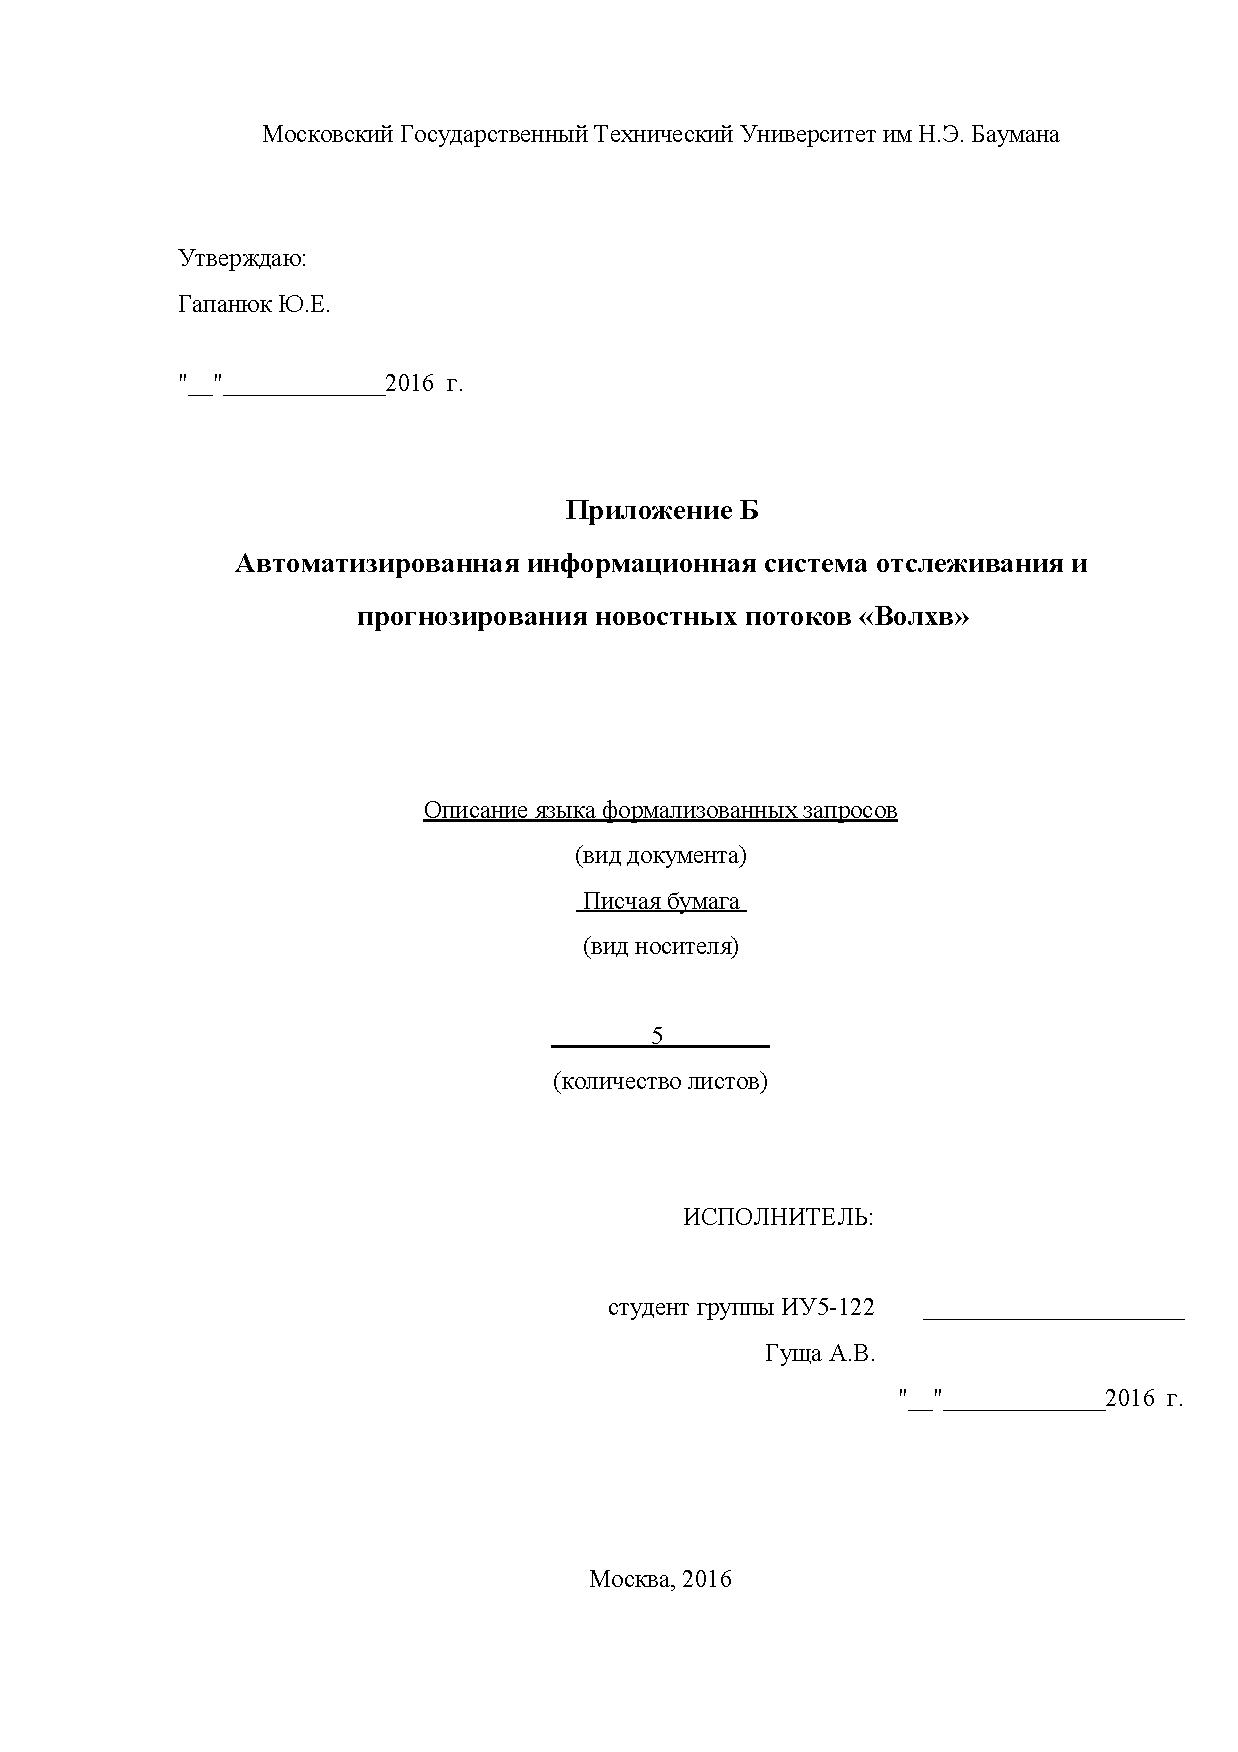
\includepdf[pages=1]{sphinx_title.pdf}
\setcounter{pageaux}{1}
\setcounter{page}{174}
\tableofcontents

\clearpage
\section{Конструкции языка запросов для полнотекстового поиска}

Формализованный язык запросов для полнотекстового поиска состоит из набора элементов, перечисленных в таблице~\ref{table:elements}.

\begin{center}
\begin{longtable}{L{6cm}|L{10cm}}
\caption{Элементы языка полнотекстового поиска}
\label{table:elements} \\
\multicolumn{1}{C{6cm}|}{Элемент языка} & 
\multicolumn{1}{C{6cm} }{Описание} \\
\hline\hline
\endhead

Слово & Поиск документов, содержащих данное слово. \\
Слово1 Слово2 & Поиск документов, содержащих хотя бы одно из слов. \\
“Слово1 Слово2” & Поиск документов, содержащих оба слова в произвольном порядке без разделяющих слов между ними. \\
Слово1 NEAR~n Слово2 & Поиск документов, содержащих оба слова в заданном порядке с максимальном количеством n слов между ними. \\
“Слово1 Слово2”~n & Поиск документов, содержащих оба слова с максимальным суммарным расстоянием между всеми словами выражения не большим n. \\
Выражение1 | Выражение2 & Поиск документов, удовлетворяющих либо выражению языка “Выражение1”, либо выражению языка “Выражение2”. \\
Слово1 MAYBE Слово2 & Поиск документов со словом “Слово1” и опциональным “Слово2”, документы с обоими словами считаются приоритетными. \\
Слово1 -Слово2, Слово1 !Слово2 & Поиск документов со словом “Слово1” и не содержащих слово “Слово2”. \\
@Поле Выражение & Поиск документов, удовлетворяющих выражению по конкретному реквизиту документа. \\
@(Поле1, Поле2) Выражение & Поиск документов, удовлетворяющих выражению по конкретным реквизитам документа. \\
@!Поле Выражение & Поиск документов, удовлетворяющих выражению, исключая конкретный реквизит из поиска. \\
@!(Поле1, Поле2) Выражение & Поиск документов, удовлетворяющих выражению, исключая конкретные реквизиты из поиска. \\
“Слово1 Слово2 Слово3”/n & Поиск документов, содержащих хотя бы n ключевых слов. \\
Слово1 <\< Слово2 & Поиск документов, содержащих оба слова в заданном порядке. \\
\begin{verbatim}^Слово\end{verbatim} & Реквизит документа должен начинаться с заданного слова. \\
Слово\$ & Реквизит документа должен заканчиваться заданным словом. \\
Слово\^n & Увеличивает приоритет слова над другими словами выражения в n раз. \\
Слово1 SENTENCE Слово2 & Слова реквизита документа должны быть в пределах одного предложения. \\
Выражение1 PARAGRAPH Выражение2 & Документ должен удовлетворять выражениям языка в пределах одного параграфа.\\

\end{longtable}
\end{center}

\section{Конструкции языка запросов для поиска по реквизитам}

Формирование критериев поиска осуществляется на клиентской стороне на основе графических форм ввода для аналитика или на основе проблемно-ориентированного языка (DSL) поиска по реквизитам.

DSL для поиска по реквизитам содержит список выражений:
\begin{equation}
@ <\text{атрибут}> <\text{операция}> <\text{поисковый критерий}> 
\end{equation}
Где атрибут может принимать значения:
\begin{itemize}
\item id -- идентификатор документа;
\item url -- источник документа;
\item timestamp -- метка времени документа;
\item title -- заголовок документа;
\item content -- содержание документа;
\item rubric -- список рубрик документа;
\item tags -- список меток документа;
\end{itemize}

Где операция может принимать значения:
\begin{itemize}
\item “=” – сравнение на совпадение значений;
\item “>” – операция «больше»;
\item “<” – операция «меньше»;
\item “>=” – операция «больше или равно»;
\item “<=” – операция «меньше или равно»;
\item “!=” – операция на несовпадение значений;
\item “IN” – операция на принадлежность множеству значений, с этой операцией значение поискового критерия задаётся кортежем вида (<значение1>, …, <значение2>);
\end{itemize}

Значение поискового критерия зависит от семантики производимого поиска.


\resetpageaux
\end{document}